\documentclass[xcolor=x11names,compress]{beamer}
%% General document %%%%%%%%%%%%%%%%%%%%%%%%%%%%%%%%%%
\usepackage{graphicx}
\usepackage{tikz}
\usetikzlibrary{decorations.fractals}
%%%%%%%%%%%%%%%%%%%%%%%%%%%%%%%%%%%%%%%%%%%%%%%%%%%%%%
%% Beamer Layout %%%%%%%%%%%%%%%%%%%%%%%%%%%%%%%%%%
\useoutertheme[subsection=false,shadow]{miniframes}
\useinnertheme{default}
\usefonttheme{serif}
\usepackage{palatino}
\usepackage{setspace,textcomp,soul}
\usepackage{listings}

\setbeamerfont{title like}{shape=\scshape}
\setbeamerfont{frametitle}{shape=\scshape}
\definecolor{cream}{RGB}{253,230,228}
\definecolor{greenBG}{RGB}{1,35,0}
\definecolor{bluUnicam}{RGB}{27,43,74}
\definecolor{redUnicam}{RGB}{219,0,36}
\definecolor{orangeUnicam}{RGB}{234,114,40}
\setbeamercolor*{lower separation line head}{bg=redUnicam} 
\setbeamercolor*{normal text}{fg=cream} 
\setbeamercolor*{alerted text}{fg=red} 
\setbeamercolor*{example text}{fg=black} 
\setbeamercolor*{structure}{fg=cream} 
\setbeamercolor*{frametitle}{fg=cream}

\setbeamercolor*{palette tertiary}{fg=cream,bg=bluUnicam} 
\setbeamercolor*{palette quaternary}{fg=black,bg=black!10} 

\setbeamercolor*{background canvas}{bg=greenBG}
%%%%%%%%%%%%%%%%%%%%%%%%%%%%%%%%%%%%%%%%%%%%%%%%%%
%% Author data and Logo %%%%%%%%%%%%%%%%%%%%%%%%%%
\subtitle{$<$Put Subtitle Here$>$}
\author[shortname]{
    {\textbf{Francesco Moschella\\}}
    {\small{w/\\}}
    {\textbf{GitHub Copilot\\}}
}

\date{
    \vspace*{-0.7cm}
	\begin{figure}[htpb!]
    	\centering
        
\includegraphics[width=0.15\textwidth]{resources/figures/utils/logo}
    \end{figure}
    \today
}

\newcommand{\red}[1]{{\color{red}#1}}

\begin{document}
%%%%%%%%%%%%%%%%%%%%%%%%%%%%%%%%%%%%%%%%%%%%%%%%%%%%%%
%%%%%%%%%%%%%%%%%%%%%%%%%%%%%%%%%%%%%%%%%%%%%%%%%%%%%%
\section{\scshape}
\begin{frame}
    \begin{center}
        \title{\color{cream}{
            \Large{Programming Methodologies}\\
            \small{Functional Programming Module}\\
            \small{Tutoring}}}
        \titlepage
    \end{center}
\end{frame}

\begin{frame}{Outline}
    \tableofcontents
\end{frame}
\begin{frame}
    \centering
    \huge{\red{\textbf{STOP ME}} if you need \red{\textbf{HELP}} or something is \red{\textbf{UNCLEAR}}}
\end{frame}
%%%%%%%%%%%%%%%%%%%%%%%%%%%%%%%%%%%%%%%%%%%%%%%%%%%%%%
%%%%%%%%%%%%%%%%%%%%%%%%%%%%%%%%%%%%%%%%%%%%%%%%%%%%%%
\section{Introduction}
\begin{frame}{Me}
    \begin{itemize}
        \item \textbf{Name}: Francesco Moschella
        \item \textbf{Email}: \href{mailto:francesco.moschella@studenti.unicam.it}{Francesco.Moschella@studenti.unicam.it}
        \item \textbf{Social}:
        \begin{itemize}
            \item \textbf{Telegram}: \href{https://t.me/HarlockOfficial}{@HarlockOfficial}
            \item \textbf{Instagram}: \href{https://www.instagram.com/HarlockOfficial}{@HarlockOfficial}
            \item \textbf{GitHub}: \href{https://www.github.com/HarlockOfficial}{@HarlockOfficial}
    
        \end{itemize}
        \item \textbf{Currently Enrolled In}: MSc in AIIR 2° Year
        \item \textbf{Interests}: Videogames, TV Series, Movies, Cartoons/Anime, Music, Alchool, Programming, ...
        \item \textbf{Availability}: Always at the coffee machine, anytime you see me in the department, text messages (except when I sleep, eat, play, work, ...)
    \end{itemize}
    Am I missing something? Let me know!
\end{frame}

\begin{frame}{Tu}
    Things I would like to know about you:
    \begin{itemize}
        \item Name
        \item Interests
        \item Hobby
        \item Main problem with the course in general (if any)
        \item Last hangover (and why?)
        \item ...
    \end{itemize}
\end{frame}
%%%%%%%%%%%%%%%%%%%%%%%%%%%%%%%%%%%%%%%%%%%%%%%%%%%%%%
\section{Environment Setup}
\begin{frame}{Environment Setup}
    Haskell Installer:
    \begin{itemize}
        \item \textbf{GHCup} (\href{https://www.haskell.org/ghcup/}{download link}) tool to install GHC, Cabal, Stack and Haskell Language Server
    \end{itemize}
    IDE Links:
    \begin{itemize}
        \item \textbf{VSCode} (\href{https://code.visualstudio.com/}{download link}) IDE
        \item \textbf{IntelliJ IDEA} (\href{https://www.jetbrains.com/idea/download/}{download link}) IDE 
    \end{itemize}
    Useful Plugins:
    \begin{itemize}
        \item \textbf{GitHub Copilot} OR any AI code completion tool
        \item \textbf{Git Lens} (VSCode only)
        \item \textbf{Haskell} (VSCode only)
        \item \textbf{IntelliJ-Haskell} (IntelliJ IDEA only)
    \end{itemize}
\end{frame}
%%%%%%%%%%%%%%%%%%%%%%%%%%%%%%%%%%%%%%%%%%%%%%%%%%%%%%
\section{Basic Concepts}
\begin{frame}{Basic Concepts}
    \begin{itemize}
        \item Haskell is a \textbf{pure} language
        \item Haskell is a \textbf{statically typed} language
        \item Haskell is a \textbf{strongly typed} language
        \item Haskell is a language with \textbf{lazy evaluation}
        \item Haskell is a language with \textbf{type inference}
        \item Everything in Haskell is a \textbf{function} (\href{https://limited.systems/articles/everything-is-a-function/}{Reference Link})
    \end{itemize}
\end{frame}
\begin{frame}{Example}
    \lstinputlisting[language=Haskell]{resources/code/lecture_01/basic_concepts/basic_example.hs}
\end{frame}
\begin{frame}{Scope}
    \begin{block}{Definition}
        The scope of a variable is the region of the program within which the variable can be accessed.
    \end{block}
    \begin{block}{Global Scope}
        Variables declared outside of a function are global variables. They can be accessed from any function in the program.
    \end{block}
    \begin{block}{Local Scope}
        Variables declared inside a function are local variables. They can be accessed only within the function in which they are declared.
    \end{block}
\end{frame}
\begin{frame}{Example}
    \lstinputlisting[language=Haskell]{resources/code/lecture_01/basic_concepts/scope_example.hs}
\end{frame}
\begin{frame}{Tuples}
    \begin{block}{Definition}
        A tuple is a collection of elements of different types. Tuples are immutable, i.e., their elements cannot be modified.
    \end{block}
    \begin{block}{Properties}
        \begin{itemize}
            \item Tuples can contain elements of different types.
            \item Tuples can contain elements of the same type.
            \item Tuples can contain zero elements.
            \item Tuples cannot contain one element.
            \item Typing information define the tuple length.
        \end{itemize}
    \end{block}
    \begin{block}{Syntax}
        \begin{itemize}
            \item Tuples are enclosed in parentheses.
            \item Elements are separated by commas.
        \end{itemize}
    \end{block}
\end{frame}
\begin{frame}{Example}
    \lstinputlisting[language=Haskell]{resources/code/lecture_01/basic_concepts/tuples_example.hs}
\end{frame}
\begin{frame}{Lists}
    \begin{block}{Definition}
        \begin{itemize}
            \item A list is a sequence of elements of the same type.
        \end{itemize}
    \end{block}
    \begin{block}{Properties}
        \begin{itemize}
            \item Lists can contain elements of the same type.
            \item Lists can contain from zero to an arbitrary number of elements.
        \end{itemize}
    \end{block}
    \begin{block}{Syntax}
        \begin{itemize}
            \item Lists are enclosed in square brackets.
            \item Elements are separated by commas.
        \end{itemize}
    \end{block}
\end{frame}
\begin{frame}{Example}
    \lstinputlisting[language=Haskell]{resources/code/lecture_01/basic_concepts/lists_example.hs}
\end{frame}
%%%%%%%%%%%%%%%%%%%%%%%%%%%%%%%%%%%%%%%%%%%%%%%%%%%%%%
\section{Functions}
\begin{frame}{Functions}
    % Haskell functions
    \begin{block}{Definition}
        A function is a \textbf{relation} between a set of \textbf{inputs} and a set of \textbf{possible outputs} with the property that each input is related to \textbf{exactly one output}.
    \end{block}
    \begin{block}{Properties}
        \begin{itemize}
            \item \textbf{Pure functions} have no side effects.
            \item \textbf{Higher-order functions} can take functions as arguments and return functions.
            \item \textbf{Recursion} is a technique in which a function calls itself.
        \end{itemize}
    \end{block}
    \begin{block}{Syntax}
        \begin{itemize}
            \item \textbf{Function definition}: \texttt{f x = x + 1}
            \item \textbf{Function application}: \texttt{f 1}
            \item \textbf{Anonymous functions}: \texttt{(\textbackslash x -> x + 1)}
        \end{itemize}
    \end{block}
\end{frame}
\begin{frame}{Example}
    \lstinputlisting[language=Haskell]{resources/code/lecture_01/functions/core_concepts_example.hs}
\end{frame}
\begin{frame}{Guards}
    \begin{block}{Definition}
        \begin{itemize}
            \item Guards are a way to define functions based on conditions.
        \end{itemize}
    \end{block}
    \begin{block}{Properties}
        \begin{itemize}
            \item Guards are evaluated from top to bottom.
            \item The first guard that evaluates to \texttt{True} is executed.
            \item The ``otherwise'' guard is optional and is executed if no other guard evaluates to \texttt{True}.
        \end{itemize}
    \end{block}
    \begin{block}{Syntax}
        \begin{itemize}
            \item Guards are defined after the function name.
            \item Guards are separated by the pipe symbol ($|$).
            \item Guards are followed by the function body.
        \end{itemize}
    \end{block}
\end{frame}
\begin{frame}{Example}
    \lstinputlisting[language=Haskell]{resources/code/lecture_01/functions/guards_example.hs}
\end{frame}
\begin{frame}{Recursion}
    \begin{block}{Definition}
        Recursion is a technique in which a \textbf{function calls itself} as a subroutine or where a \textbf{set of functions call each other in a circular chain}.
    \end{block}
    \begin{block}{Base Case (Not mandatory, but highly recommended)}
        A recursive function should have a base case that terminates the recursion.
    \end{block}
    \begin{block}{Self-Recursive Case}
        A recursive function can have a recursive case that calls itself, hopefully with a modified (smaller) input.
    \end{block}
    \begin{block}{Circular Recursion}
        A recursive function can have a case where calls another function, which in turn may call other functions that call the first one.
    \end{block}
\end{frame}
\begin{frame}{Example}
    \lstinputlisting[language=Haskell]{resources/code/lecture_01/functions/recursion_example.hs}
\end{frame}
\begin{frame}{Lambda Functions}
    \begin{block}{Definition}
        \begin{itemize}
            \item Are anonymous function.
            \item Are functions defined without a name.
        \end{itemize}
    \end{block}
    \begin{block}{Properties}
        \begin{itemize}
            \item Are used to define simple functions.
            \item Are used to define functions that are used only once.
            \item Are used to define functions that are passed as arguments to other functions.
        \end{itemize}
    \end{block}
    \begin{block}{Syntax}
        \begin{itemize}
            \item Are defined using the ``\textbackslash'' symbol.
            \item Are followed by the function arguments.
            \item Are followed by the function body.
        \end{itemize}
    \end{block}
\end{frame}
\begin{frame}{Example}
    \lstinputlisting[language=Haskell]{resources/code/lecture_01/functions/lambda_example.hs}
\end{frame}
\begin{frame}{Pattern Matching}
    \begin{block}{Definition}
        Pattern matching is a way to check a value against a pattern.
    \end{block}
    \begin{block}{Properties}
        \begin{itemize}
            \item It is a more powerful version of the switch statement in C.
            \item It is a more powerful version of the if-else statement in C.
            \item It is a more powerful version of the ternary operator in C.
            \item It is often used with guards.
            \item It is often used with recursion.
        \end{itemize}
    \end{block}
\end{frame}
\begin{frame}{Example}
    \lstinputlisting[language=Haskell]{resources/code/lecture_01/functions/pattern_matching_example.hs}
\end{frame}
\begin{frame}{Partial Application}
    \begin{block}{Definition}
        \begin{itemize}
            \item A function is partially applied when it is called with fewer arguments than it expects.
        \end{itemize}
    \end{block}
    \begin{block}{Properties}
        \begin{itemize}
            \item Is a way to create new functions from existing functions.
            \item Is a way to create functions with fewer arguments.
            \item Is a way to create functions with default arguments.
        \end{itemize}
    \end{block}
    \begin{block}{Syntax}
        \begin{itemize}
            \item Is done by passing fewer arguments than the function expects.
        \end{itemize}
    \end{block}
\end{frame}
\begin{frame}{Example}
    \lstinputlisting[language=Haskell]{resources/code/lecture_01/functions/partial_application_example.hs}
\end{frame}
\begin{frame}{Higher Order Functions}
    \begin{block}{Definition}
        \begin{itemize}
            \item Are functions that take other functions as arguments.
            \item Are functions that return functions as results.
        \end{itemize}
    \end{block}
    \begin{block}{Properties}
        \begin{itemize}
            \item Are used to define functions that are passed as arguments to other functions.
        \end{itemize}
    \end{block}
\end{frame}
\begin{frame}{Example}
    \lstinputlisting[language=Haskell]{resources/code/lecture_01/functions/higher_order_example.hs}
\end{frame}
%%%%%%%%%%%%%%%%%%%%%%%%%%%%%%%%%%%%%%%%%%%%%%%%%%%%%%
\section{Typing}
\begin{frame}{Type System}
    \begin{block}{Definition}
        \begin{itemize}
            \item A type system is a tractable syntactic method for proving the absence of certain program behaviors by classifying phrases according to the kinds of values they compute.
        \end{itemize}
    \end{block}
    \begin{block}{Properties}
        \begin{itemize}
            \item It is a way to ensure that a program behaves as expected.
            \item It is a way to ensure that a program is correct.
            \item It is a way to ensure that a program is safe.
            \item It is a way to ensure that a program is secure.
        \end{itemize}
    \end{block}
\end{frame}
\begin{frame}{Example}
    \lstinputlisting[language=Haskell]{resources/code/lecture_01/typing/type_system_example.hs}
\end{frame}
\begin{frame}{Currying}
    \begin{block}{Definition}
        Currying is the technique of translating the evaluation of a function that takes multiple arguments into evaluating a sequence of functions, each with a single argument.
    \end{block}
\end{frame}
\begin{frame}{Example}
    \lstinputlisting[language=Haskell]{resources/code/lecture_01/typing/currying_example.hs}
\end{frame}
\begin{frame}{Polymorphism}
    \begin{block}{Definition}
        Polymorphism is the ability of a function to behave ``correctly'' on different data types.
    \end{block}
    \begin{block}{Properties}
        \begin{itemize}
            \item Polymorphism is a key concept in functional programming.
            \item Polymorphism allows for the definition of functions that can be applied to a range of data types.
        \end{itemize}
    \end{block}
\end{frame}
\begin{frame}
    \centering
    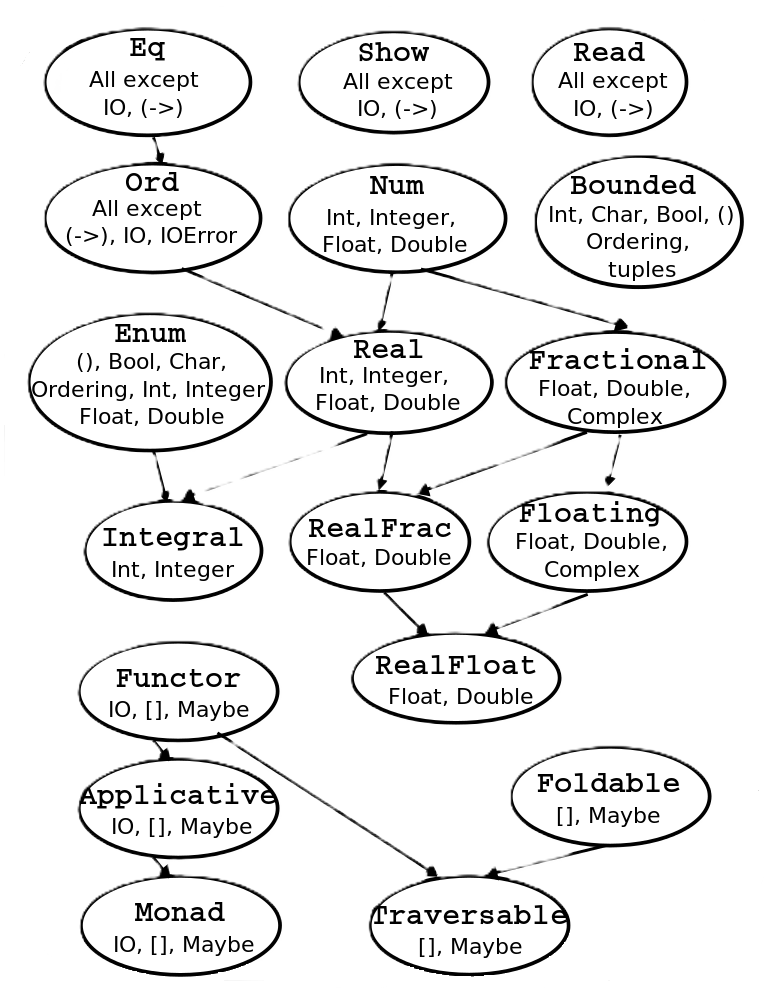
\includegraphics[height=.8\textheight]{resources/figures/lecture_01/typing/Base_classes_hierarchy.png}
    {\tiny \url{https://en.wikibooks.org/wiki/Haskell/Classes_and_types}}
\end{frame}
\begin{frame}{Example}
    \lstinputlisting[language=Haskell]{resources/code/lecture_01/typing/polymorphism_example.hs}
\end{frame}
\begin{frame}{Type Classes}
    \begin{block}{Definition}
        Type classes are a construct that allows for ad-hoc data types definition.
    \end{block}
\end{frame}
\begin{frame}{Example}
    \lstinputlisting[language=Haskell]{resources/code/lecture_01/typing/type_classes_example.hs}
\end{frame}
%%%%%%%%%%%%%%%%%%%%%%%%%%%%%%%%%%%%%%%%%%%%%%%%%%%%%%
\section{Monads}
\begin{frame}{Monads}
    \begin{block}{Definition}
        Monads are a design pattern that allows for the composition of functions that return a monadic value.
    \end{block}
    \begin{block}{Properties}
        \begin{itemize}
            \item Monads are a key concept in functional programming.
            \item Monads allow for the definition of functions that can be applied to a range of data types.
        \end{itemize}
    \end{block}
\end{frame}
\begin{frame}{Example}
    \lstinputlisting[language=Haskell]{resources/code/lecture_01/monads/monads_example.hs}
\end{frame}
%%%%%%%%%%%%%%%%%%%%%%%%%%%%%%%%%%%%%%%%%%%%%%%%%%%%%%
\section{Type Inference}
\begin{frame}{Type Inference}
    \begin{block}{Definition}
        Type inference is the process of determining the type of an expression in a programming language.
    \end{block}
    \begin{block}{Rules}
        \begin{enumerate}
            \item The type of a variable is the type of the value it is bound to.
            \item The type of a function is the type of its arguments and return value.
            \item The type of an expression is the type of the value it evaluates to.
        \end{enumerate}
    \end{block}
\end{frame}
\begin{frame}
    \begin{block}{Steps}
        \begin{enumerate}
            \item Assign every variable a unique type variable.
            \item Assign every function its type with new unique type variables.
            \item For each subexpression of the expression, generate equations of types.
            \item Resolve the equations until no further simplification is possible.
        \end{enumerate}
        NOTE: Conflicting types imply a type error, otherwise the expression is well-typed and the type has been inferred.
        \url{https://www.youtube.com/watch/bv7aenMgSkg}
    \end{block}
\end{frame}
\begin{frame}{Example}
    \lstinputlisting[language=Haskell]{resources/code/lecture_01/type_inference/type_inference_example.hs}
\end{frame}
% NOTE: These last topics may require more slides
%%%%%%%%%%%%%%%%%%%%%%%%%%%%%%%%%%%%%%%%%%%%%%%%%%%%%%
%%%%%%%%%%%%%%%%%%%%%%%%%%%%%%%%%%%%%%%%%%%%%%%%%%%%%%
\section*{}
\begin{frame}{}
\begin{center}

\includegraphics[width=6.5cm]{resources/figures/utils/thanks}
\end{center}
\end{frame}
%%%%%%%%%%%%%%%%%%%%%%%%%%%%%%%%%%%%%%%%%%%%%%%%%%%%%%
%%%%%%%%%%%%%%%%%%%%%%%%%%%%%%%%%%%%%%%%%%%%%%%%%%%%%%
\end{document}
